\documentclass[a4paper,12pt]{report}

\usepackage[utf8]{inputenc}
\usepackage[english]{babel}
\usepackage{natbib}
\usepackage[T1]{fontenc}
\usepackage{setspace}
\usepackage{graphicx}
\usepackage{hyperref}
\usepackage{csquotes}
\usepackage[top=3.5cm,left=2.5cm,right=2.5cm,bottom=3.5cm]{geometry} % 'showframe' to see borders

\graphicspath{ {images/} }

\def \reportTitle{Recommending photo filters via image content in a Web App \& REST API}

\title{\vspace{-2cm}
\includegraphics[width=5cm]{mmu-white.pdf}\\\vspace{4cm}\reportTitle\vspace{1cm}}

\author{Joshua Bridge\\14032908\\joshua.m.bridge@stu.mmu.ac.uk}

\begin{document}

\maketitle

\doublespacing

\begin{abstract}
  \textit{To be completed.}
\end{abstract}

\tableofcontents

\listoffigures

\listoftables

\chapter{Introduction}
  % TODO Complete summary of introduction
  % ADD

  \newpage

  \section{Aims}
    In this report the following goals are what is expected to be achieved in the creation of the product:

    \begin{enumerate}
      \item To reduce complexity, information overload, and time spent for users when trying to customise photographs - usually in the expectation that the photographs will later be shared on social media.
      \item To create a secure platform for other applications to utilise the advancements made in this project.
    \end{enumerate}

  \section{Objectives} \label{sec:objectives}
    The objectives below describe in more detail a set of more specific goals which should be achieved in order to create a successful product:

    \begin{enumerate}
      \item \label{obj1}Implement a simple online web application for filtering images using a framework or library designed for front-end development across multiple platforms.
      \item \label{obj2}Implement a back-end application which is able to process images including applying filters and creating thumbnails.
      \item \label{obj3}Research various recommender systems to determine the common technologies/solutions for solving the problem of recommendations.
      \item \label{obj4}Implement a recommender system which is able to suggest photo filters to users based on image content.
      \item \label{obj5}Implement a RESTful API which exposes both the recommender system and the filtering system to the front-end web app and allows developers to connect them into their own applications.
    \end{enumerate}

  \section{Digital image processing}
   Image processing deals with the analysis and manipulation of image data. An example of image processing is the use of digital signal processing. This involves converting analog sensory data from a digital camera sensor into a computer-interpretable format with minimal data loss from external sources such as noise and distortion.\\

   \subsection{Bitmaps}
     Before you are able to analyse an image, you must first represent the data in a way that it can be interpreted by a computer, and a human. One basic form of doing this is via a bitmap image. A bitmap - as its name implies - is a simple spacial mapping of values (bits) along a horizontal axis (x) and vertical axis (y). Using a greyscale image as an example, a bitmap representation of this would contain a number of values (or ‘pixels’), the number of which is equal to the product of the sizes of the x and y axis. Therefore an image of size 200 x 200 would contain 40,000 pixels. Each of these pixels contains an integer value representing brightness, typically ranging from 0 - 255 (the total value range of an 8-bit integer), ‘0’ being completely black, ‘255’ being completely white.

     A colour image follows a very similar format, except now each pixel contains three brightness values instead of one. Each of these values map to the brightness of the colours (or ‘channels’) red, green and blue - in that order. Therefore a pixel with values (0,255,0) would be entirely green and a pixel with values (0,0,255) would be entirely blue. It should be noted that when these colours are displayed on a computer screen their colour values are additive (i.e. they can mix together to form a different, brighter colour). A pixel with values (0,255,255) would therefore represent cyan, and finally a pixel with values (255,255,255) would represent white.

   \subsection{Image processing tasks}
     There are several methods of improving the results of image analysis, one of which is to run an image processing algorithm against it. Generally this is to make the image clearer by sharpening it or removing noise - these are often referred to as low-level processing methods \citep{sonka2014image}. While these methods are often applied to make analysis by a computer a lot easier, they also can be used to increase the ‘clarity’ or the percieved ‘beauty’ of an image when viewed by a human.

     \subsubsection{Sharpening}
       For an image to be captured, it must first enter through some kind of lens which refracts the incoming light into a ‘focal point’ onto which some kind of light-sensitive surface is placed such as a digital image sensor. In order for an object to be perfectly ‘in focus’ it must be at the optimal distance from the lens - an area known as the ‘focal plane’. If the subject of a photograph is not near enough to the focal plane (either in front of it or behind it) then the subject will appear to blur.

  \section{Computer vision}
   Computer vision involves modelling the human vision system in such a way that a computer can interpret abstract visual data.

\chapter{Literature Review}

  In order to understand the background of the technology involved in this project, it is necessary to complete a significant review into the current and past literature. This will help form a basis of knowledge from which the future development and analysis of the proposed system will utilise and build upon. This research will be vital in order to make use of the most optimal technology for any given problem.

  The following review will be an investigation into the current knowledge of the major components of the proposed system, which are as follows:

  \begin{itemize}
    \item The recommendation system.
    \item The image filtering system.
    % \item The web-based user interface.
  \end{itemize}

  \section{Recommendation systems} \label{sec:lit-recc}
    As defined in \cite{ricci2011introduction}, recommending content is a problem which involves attempting to predict what a user may desire at any given time when using a system. In the ‘internet era’ applications of this are far-reaching, such as recommending products on Amazon.com \cite{linden2003amazon}. Recommendation systems are a popular topic due to the \textquote{abundance of practical applications that help users to deal with information overload and provide personalized recommendations, content, and services to them} \citep{adomavicius2005toward}.

    \cite{jannach2010recommender} describe three different methods for giving recommendations: Collaborative, Collaborative, Content-based, and Hybrid.

    \subsection{Collaborative recommendation}
      When using an online streaming platform that serves video content such as Netflix or YouTube, a user will visit their site looking for something to watch. The problem faced by these sites is trying to find content that the user hasn't seen before, but will align with the user's interests enough to make them want to watch it \citep{davidson2010youtube}, \citep{gomez2016netflix}.
      The information needed to carry out such a prediction can include the semantic value of the entire users history of interaction with the system (often referred to as \textit{metadata} \citep{duval2002metadata}), from which preference can be extrapolated. If there is not enough metadata about the user from which to extrapolate preference with reasonable certainty, then preference can be inferred from other users of the system - especially users with a similar predicted preference.

    \subsection{Content-based recommendation}
      There can sometimes be barriers to using collaborative recommendation, such as when the ‘cold-start problem’ is present. This problem describes when a user has just signed up to a website, it will not yet have enough information / user history to recommend them content \citep{schein2002methods}.
      In this situation content-based recommendation could be used more effectively to build up more reliable recommendations \citep{lops2011content}.
      There are different kinds of content-based recommendation, as it can be applied to many different kinds of content. For example a system may work differently if the content is user-generated as opposed to internally or computer generated, where the information would likely be provided already. In a system with user-generated content, the information about that content would have to be inferred, or provided by the user.

      \subsubsection{Feature extraction for content analysis}
        When content is user-generated and without a definition provided alongside it, its definition must be derived. For textual data this can be done by analysing the words and extrapolating a commonality between keywords to find a prevailing subject \citep{sanderson1999deriving}.
        This type of process is often referred to as ‘Feature extraction’ \citep{guyon2006introduction}.
        When analysing raw data such as an image file or an audio file, this becomes a much more difficult task as you must first find a way of deciphering the content before deriving the subject or meaning.

        Deep learning has recently become a common way of deciphering this content, including for image, audio, and video content types \citep{coates2011analysis}, \citep{ciregan2012multi}, \citep{lee2009unsupervised}, \citep{mobahi2009deep}.
        Spotify has implemented this kind of deep learning to determine genre types from raw audio data - see section \ref{discoverweekly}.
        This can be applied to image data also, for example in the context of a search algorithm, it would bring the most relevant images by content to the top of the results \citep{yee2003faceted}. This works similarly to how a recommender system will select the most relevant items for the user to see.

        Google's ImageNet has proven to be a very reliable system for image classification \citep{krizhevsky2012imagenet}.
        As it has a very high accuracy on most image types, it would be reasonably effective for providing a basis of feature extraction for use in a recommender system. In the system proposed in this report, scene classification along with prevailing colours in the image would be an ideal input into the recommendation system for determining optimal image filters.

        % TODO more on ImageNet

    \subsection{Hybrid recommendation}
      Generally, hybrid recommendation applies both of the previous methods together in order to draw up a more comprehensive list of recommendations, in order to avoid the individual weaknesses of both types.

      \subsubsection{Spotify - Discover Weekly}
      \label{discoverweekly}
        Discover Weekly is a playlist made every week for every user of Spotify. Instead of getting humans to curate a playlist for each and every user, an algorithm is used to try and find a set of songs which it predicts the user will like, but hasn't listened to before. As described by \cite{popper2015dw} it does this by mixing collaborative and content-based recommendation. The first is done by analysing all playlists on spotify and determining their similarity to playlists made by the user. The next step is looking for songs in those playlists that the user in question hasn't heard yet.

        \begin{figure}[ht]
          \centering
          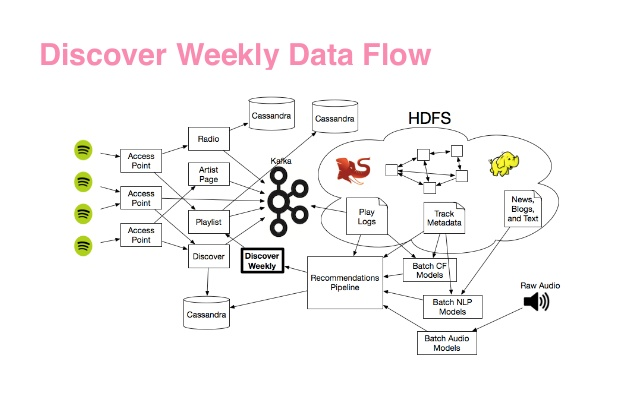
\includegraphics[width=\linewidth]{discoverweekly-dataflow}
          \caption[System component architecture of Spotify's ‘Discover Weekly’]{System component architecture of Spotify's ‘Discover Weekly’ \protect\citep{johnson2015dw}}
          \label{fig:discoverweekly-dataflow}
        \end{figure}

        The second, more complicated part of this process is the content-based recommendation. Spotify's algorithms actually analyse the music data in several different ways to determine a users ‘taste’. The first is by defining the genres a user listens to, which it does by scanning music blogs for what genre a certain piece of music is described as being. Using this as a search, spotify can then look for other music in that genre to recommend. The arguably more complicated part of this process is the auditory analysis of raw music data. As shown in figure \ref{fig:discoverweekly-dataflow} the raw audio is converted into ‘batch audio models’ where they can be used as a basis for recommendations.

      % \subsection{Image classification in recommendations}

  \section{Image filtering system}
    There is little to no research into the area of developing new photo filters, likely due to the fact that filters can be very subjective in terms of what effect they have on an image. Furthermore the relation of that effect to how many people choose that filter for a certain type of photograph would require a large data-set. However it is possible to determine the most common types of photographs posted online, which will guide the process of creating filter templates.

    \subsection{Instagram} \label{sec:lit-insta}
      In order to create image filters that users would want to apply to their photographs, an assessment must first be made about that the type of photos people tend to post online. ‘Instagram’ is a popular online photo-sharing platform that attracts over 700 million users \citep{instagram2017users}. An investigation by \cite{hu2014we} revealed that the types of photos posted on Instagram could be roughly categorised into eight types: \textquote{self-portraits, friends, activities, captioned photos (pictures with embedded text), food, gadgets, fashion, and pets}. The study clarifies that ‘self-portraits’ (or ‘selfies’) made up 24.2\% of the images posted, and ‘friends’ made up 22.4\%, totalling 46.6\% of the images analysed. From this it can be hypothesized that creating filters which are complimentary for skin-tones would be a contributing factor to success when developing image-filters.

      \cite{hu2014we} however did not study a wide proportion of the Instagram user-base, in fact they only closely studied 50 users, out of an initial 95,343 ‘unique seed users’, from a user-base of more than 150 million when the study was taken place. Furthermore the study only analyses pictures posted online, to Instagram, with public profiles, and from users which had \textquote{at least 30 friends, 30 followers, and had posted at least 60 photos}. The system proposed in this report would not be limited in terms of where the resulting image would be posted, and has no requirement that the image be posted to an online website. Therefore the findings in the study should only be used as a loose guideline for popular image categories when defining image-filter styles.

    \subsection{Personalisation of image enhancement}
      There has been some work done on the mapping of image enhancement styles to personal taste, although the field appears to be still in early stages. However, two studies in particular have heavily contributed to the development in this field. \cite{kang2010personalization} found that when given a set of images, participants would deviate into different styles when asked to choose between two options of enhancement (e.g. lighter or darker). Furthermore, many participants preferred their own enhancement when compared to an averaged enhancement, suggesting that personalised enhancements would be a valuable tool.

      Using the work done by \cite{kang2010personalization} as a basis, \cite{caicedo2011collaborative} developed a method of personalised image enhancement that focused on putting users into groups (or ‘clusters’) that had similar tastes within image enhancement. Therefore when attempting to apply personalised enhancement on a per-user basis, instead of determining a specific users preference from scratch, the user's preference would only have to be mapped to a pre-defined group. Using this method the authors suggest that personalisation of image enhancement could be scale-able to large amounts of users.

  % \section{Web-based user interface}

  \newpage

  \section{Conclusion}
    Posting images online is fast becoming one of the biggest trends in recent history, as evidenced by Instagram's user-base expanding to over 700 million users \citep{instagram2017users}. While not much public research seems to have been carried out into the reasons why users pick certain styles of image-filters before posting, it certainly appears viable to aid them in making that process easier.
    The findings of this review suggest that feature extraction could be a useful tool in developing recommendations for filters. This would be carried out in the form of image classification, most commonly to determine whether a person is present in a photograph which would thereby influence the algorithm's decision of what filters to recommend to the user for a certain image.

    The findings of this report also suggest (mostly from \cite{kang2010personalization} and \cite{caicedo2011collaborative}) that the field of personalised image enhancements (or filters) is a relatively new field of study, therefore there is a lot of room for collecting new findings by extending upon previous works in a new implementation.

\chapter{Design}
  In this chapter a detailed description of the product design will be laid out, including explanations for each choice of technology and how it will enable the product to achieve its goal. The product can essentially be split up into two major components - a RESTful API \& a web-based front-end. Creating an API is an important factor in the implementation as it defines how the flow of the client application will work. As a result, technologies must be chosen which easily make use of this type of application-flow such as a framework which integrates well with AJAX calls - a common way of connecting to APIs. The front-end development is also a crucial part of the implementation as it acts as a testing interface for the API. If the API is not structured well then designing a front-end around it is much more difficult, meaning any future developers wishing to use it might be dissuaded by its complexity and end up choosing a different service. Developing both at the same time makes it much easier to see how clients will access the service, therefore making it much easier to remove any complexity it may contain while the service is still being built.

  \section{Requirements} \label{sec:requirements}
    The application proposed in this report would be best utilised on multiple platforms \& devices, as the service it would offer is platform-independent (i.e. all you need is an image file). For this reason the primary focus will be making an online web-app, which connects to a seperate REST \citep{fielding2000architectural} API which performs the main functions of the application, without the clutter of the front-end mixing in with it. This would also allow other apps and services to utilise this API and integrate it with other apps, such as on social media apps when sharing an image.

    When designing a user-facing website and an API, there are certain considerations that have to be met, such as data security and ease of use. The following features define what the final product should achieve:

    \begin{itemize}
      \item A web-based user interface.
      \item A user-history (metadata) tracking mechanism.
      \item A RESTful API which can be utilised by any application.
    \end{itemize}

    Following these features, these are some of the things that should be taken into consideration when implementing these features:

      \begin{itemize}
        \item The application \& API should be relatively scalable with user traffic.
        \item It should not store any more information about users than it has to.
        \item It should maintain a reasonable level of security to prevent user-data from being stolen.
        \item It should not store user images after the user has finished using the application.
      \end{itemize}

    \section{API}
      The API is to be written in Python (\url{https://www.python.org}) due to its high suitability for dealing with image data, web-access and recommender algorithms. The application is able to be completely self-contained as it can perform all of the functions required in a single project.

      \subsection{REST / JSON}

      \subsection{Web Framework}
        A simple framework for handling HTTP access to the API endpoints is critical when creating an application which is meant to be able to handle high-volume traffic. Flask (\url{http://flask.pocoo.org}) performs exactly this purpose as it is a very lightweight framework which provides very easy methods for transferring data in different formats such as JSON.

        Other frameworks could be considered for this purpose, however few match Flask in terms of low complexity and ease-of-use. Django (\url{https://www.djangoproject.com}) is another very common web framework for Python which comes with many useful features such as a built-in user system. Many of the features, however, are not required within this project and would only increase the complexity of the code in the application. When applying the LSD methodology  \citep{poppendieck2003lean} this would come under the heading of eliminating waste - for example spending less time learning a complex framework and more time actually developing core features \& meeting requirements. Therefore Flask is a good foundation upon which to build a RESTful API that is easy to use \& easy to develop.

      \subsection{Database Storage} % mongodb
        A database is a crucial component within an application therefore choosing a suitable one is an important step in creating an application. The choice of database technology falls into a few categories such as SQL/NoSQL (or Relational/Non-Relational). There are several differences between these database types such as ability to scale and the types of data which can or should be stored by them. Non-relational databases are useful when the data to be stored is not of a strong structure, where relational databases are more suited for structured, related information. For example a relational database would be well suited for storing products on an online store, where different data such as products or orders can be stored in different tables, with connecting foreign keys. SQL databases are also very good at managing consistency e.g. when data is inserted into a table, there will definitely only be one entry input into the database. This is in comparison to NoSQL where horizontal scaling causes there to be a higher chance of duplicate entries, in an effort to ensure no data is lost while maintaining fast transaction speeds.

        NoSQL databases are often easier to host than SQL databases due to their ability to scale horizontally \citep{cattell2011scalable} rather than just vertically (i.e. adding more servers to handle load rather than upgrading from one machine to another higher power machine). This is applicable in the context of this project as a requirement (see section \ref{sec:requirements}) is that the application should be able to scale well with more users.

        When considering the type of data which needed to be stored by the application a NoSQL database seems to be best due to the non-relational types of data to be stored such as API responses. Furthermore speed is a key part as every bit of processing has to be done fast enough for the client not to time out waiting for a response. MongoDB (\url{https://www.mongodb.com}) is a popular NoSQL database with easy connectivity to python using the library pymongo (\url{https://api.mongodb.com/python/current/}). MongoDB is very fast with access speeds of up to 10 times faster than MySQL \citep{han2011survey} and also comes with a strong query language therefore it is highly suited for use in the application.

      \subsection{Image Filtering}
        The main bulk of processing done in the API can be broken down into three main components which are filtering, analysis, and recommendation. Filtering is the first step and will involve work to create multiple different photo filters which can be applied to any image which gets submitted to the API. Due to pythons ability to manipulate image data well using several different libraries such as NumPy (see section \ref{sec:numpy}) and Pillow (see section \ref{sec:pillow}).

        When an image enters processing it can be loaded into python using Pillow which creates an array containing each pixel value within the image. The pillow library provides many default methods for manipulating images such as changing brightness or contrast. Furthermore it contains methods which allow it to be transferred to different datatypes such as a NumPy array, where other kinds of mathematical operations can be applied to the pixel data such as linear interpolation. The image can also then be split into three different arrays with one for each colour channel of red, green, \& blue and then operations can be applied individually to create a colour effect on the image. For example if the red channel only was brightned by increasing each pixel value by a certain amount, then when the channels were put into a single image again this would give the image a red tint, which could be desirable for use as a filter.

        Due to the nature of the application trying to recommend filters, it would stand to reason that the filters in the application should be easily distinguishable to ensure maximum seperability between them. When being entered to the AI component (see section \ref{sec:mlp}) it is much better to have high seperability between classes (or filters) in order to find the relationship between input data and its classification.

      \subsection{Image Analysis}
        The second stage of processing (though not related to the first stage) is to analyse the image in order to gather input information for the recommendation algorithm. Providing raw pixel data would not be ideal when processing larger images as this will likely increase processing time greatly. When trying to build a dataset for use in training the recommendation algorithm it would not be ideal to store every picture input into the application as this violates one of the requirements in section \ref{sec:requirements}. Furthermore the raw pixel data will not provide extracted meaningful information such as dominant colours and face detection. Therefore, the best way to proceed is to extract and store information about the image itself without storing any actual image content. As found in section \ref{sec:lit-insta} self-portraits are a highly common type of image posted online so it could be meaningful to extract whether an image contains one or more faces in it. This information could affect how someone chooses which filter they would like to apply to an image so it is vital in this application to include this information. A link between a person in a photograph and the filter being chosen could exist if one of the filters was more complimenting to skin tones for example. In order to find the dominant colours in the image and apply face detection two different methods will be applied and are described below.

        \subsubsection{Dominant colours: K-Means} \label{sec:kmeans}
          K-Means clustering \citep{macqueen1967some} is a form of machine learning which performs a mathematical analysis on un-labeled data in order to find common groupings within that data. The number of clusters (or groupings) is first specified and the algorithm then splits the data points into that number of groups and then finds an average value for each cluster. K-Means has been used for image segmentation \citep{coleman1979image,shi2000normalized} which is an important part of computer vision. In this case K-Means clustering will be used to find the dominant colours within the image along with their amount of use within the image as a percentage. The colours found from this process will likely not be exactly as they appear in the image due to the averaging of each colour cluster to find the most common groups of colours.

          The K-Means algorithm used in this application will not need to be implemented as there is one provided by the scikit-learn library (\url{http://scikit-learn.org/stable/}) which meets all requirements and makes it easier to implement K-Means directly into the application.

        \subsubsection{Face detection: Google Vision API} \label{sec:visionapi}
          The Google Vision API (\url{https://cloud.google.com/vision/}) is a useful tool for performing a variety of image analysis steps such as face detection and logo detection. It can be accessed via a REST API using JSON as the request language therefore it should integrate into the application with relative ease using the libraries available in python such as ‘requests’ (\url{http://docs.python-requests.org/en/master/}). Google has not published what technology exactly powers the vision API other than saying in a blog post that it is run using machine learning and TensorFlow (\url{https://www.tensorflow.org}) \citep{vision2015blog}. However, due to the complex nature of face and logo detection it can be assumed that the systems behind the API are running some very complex machine learning models which require a lot of processing power to run. With this in mind it will be much simpler to integrate this API into the application rather than try to implement a custom version of face detection into the application.

      \subsection{Recommendation}
        The final stage of processing within the application is to get the recommendation for which filter would be best applied to the image.
        As discovered in section \ref{sec:lit-recc} a good way of doing this is to use neural networks in order to build a relationship between input data and a possible classification. Within this application a form of hybrid recommendation will be used whereby the input to the algorithm will be the results from image analysis as discussed in the previous section. In order to find a relationship between this data and a filter, some data will have to be provided by some initial prototype users in which they will choose a filter for a set of photos of their own choosing.

        Using the stored image analysis data as parameters and the chosen filters as classifiers, a machine learning model can be built which hopefully finds a significant link between image content and the filters which could get applied to them. This is a form of hybrid recommendation as the users interests are powering the recommendation but that information is linked directly to the content of the image, thereby mixing collaborative and content-based recommendation. However, this is not strictly including collaborative recommendation as the users are not being recommended based on tastes of similar users, but more that the collective users are helping to power the content-based recommendation.

        \subsubsection{Multi-Layer Perceptron} \label{sec:mlp}
          Multi-layer Perceptrons \citep{minsky2017perceptrons} are a type of neural network which can be used for classifying non-linearly separable data. A multi-layer perceptron consists of 1 input layer, 1 output layer and 1-to-many hidden layers which contain neurons that perform an activation function on their inputs. In the case of this application the multi-layer perceptron will be used as a recommendation algorithm by ‘learning’ the connection between image content and image filters. While it may not be best suited for recommendation in place of deep learning for example (section \ref{sec:lit-recc}), the MLP is already implemented in scikit-learn (\url{http://scikit-learn.org/stable/}) and therefore will be much easier to integrate within the application. Furthermore supervised deep-learning is more suited to dealing with pixel data, which this application aims to not keep therefore training a deep-learning model would be much more difficult without linking it to the application beforehand.

    \section{Front-end}
      A front-end is an ideal way to create a testing interface for the API and is a way to advertise to potential users of the API. Therefore one should be built which is capable of running on multiple platforms including mobile phones and desktops. This is so that it is accessible to as many people as possible, by removing as many impedences to accessing the application as possible. The most suitable way of achieving this would be to make the front-end a web-based service which could scale to various screen sizes, and thereby making the application accessible with no downloads required.

      \subsection{Frameworks \& Libraries} % React
        To achieve the best results in terms of aesthetics, functionality and work-effort, a front-end JavaScript framework is ideal for achieving the best results in the shortest time. Their pre-made code structures often eliminate a lot of the grunt work from creating reactive user interfaces from scratch, therefore they are an obvious choice.

        While there is little in the way of academic comparisons between JavaScript frameworks as told by \cite{graziotin2013making}, a subjective comparison can be made to find the most suitable framework for this application. The two commonly used libraries/frameworks are React and Angular and are discussed below.

        ReactJS (\url{https://reactjs.org}) is a JavaScript library for creating user interfaces which was created by Facebook (\url{https://www.facebook.com}). As it is entirely in JavaScript and introduces a component structure which updates when any data state changes, it is a simple way to add lots of functionality in a short time. AngularJS (\url{https://angularjs.org}) is another JavaScript library however it is not the recommended version of angular which is Angular 4 (\url{https://angular.io}) and is a framework rather than a library. Angular 4 uses typescript which could introduce complexity and the framework comes with a lot of baggage which brings a steeper learning curve as discussed by \cite{neuhaus_2017}.

        ReactJS is the library which will be used in this application due to its flexibility and ease of use with a relatively small learning curve. React Native (\url{https://facebook.github.io/react-native/}) is the variant which shall be used which allows the client to be run completely on its own without another server technology underneath it. This is commonly used to build mobile apps (as stated on the website) therefore it is highly suited for the requirements of this application, as long as the final product is able to easily scale between different browser sizes including desktop and mobile browsers.

    \section{Deployment}

      \begin{figure}[ht]
        \centering
        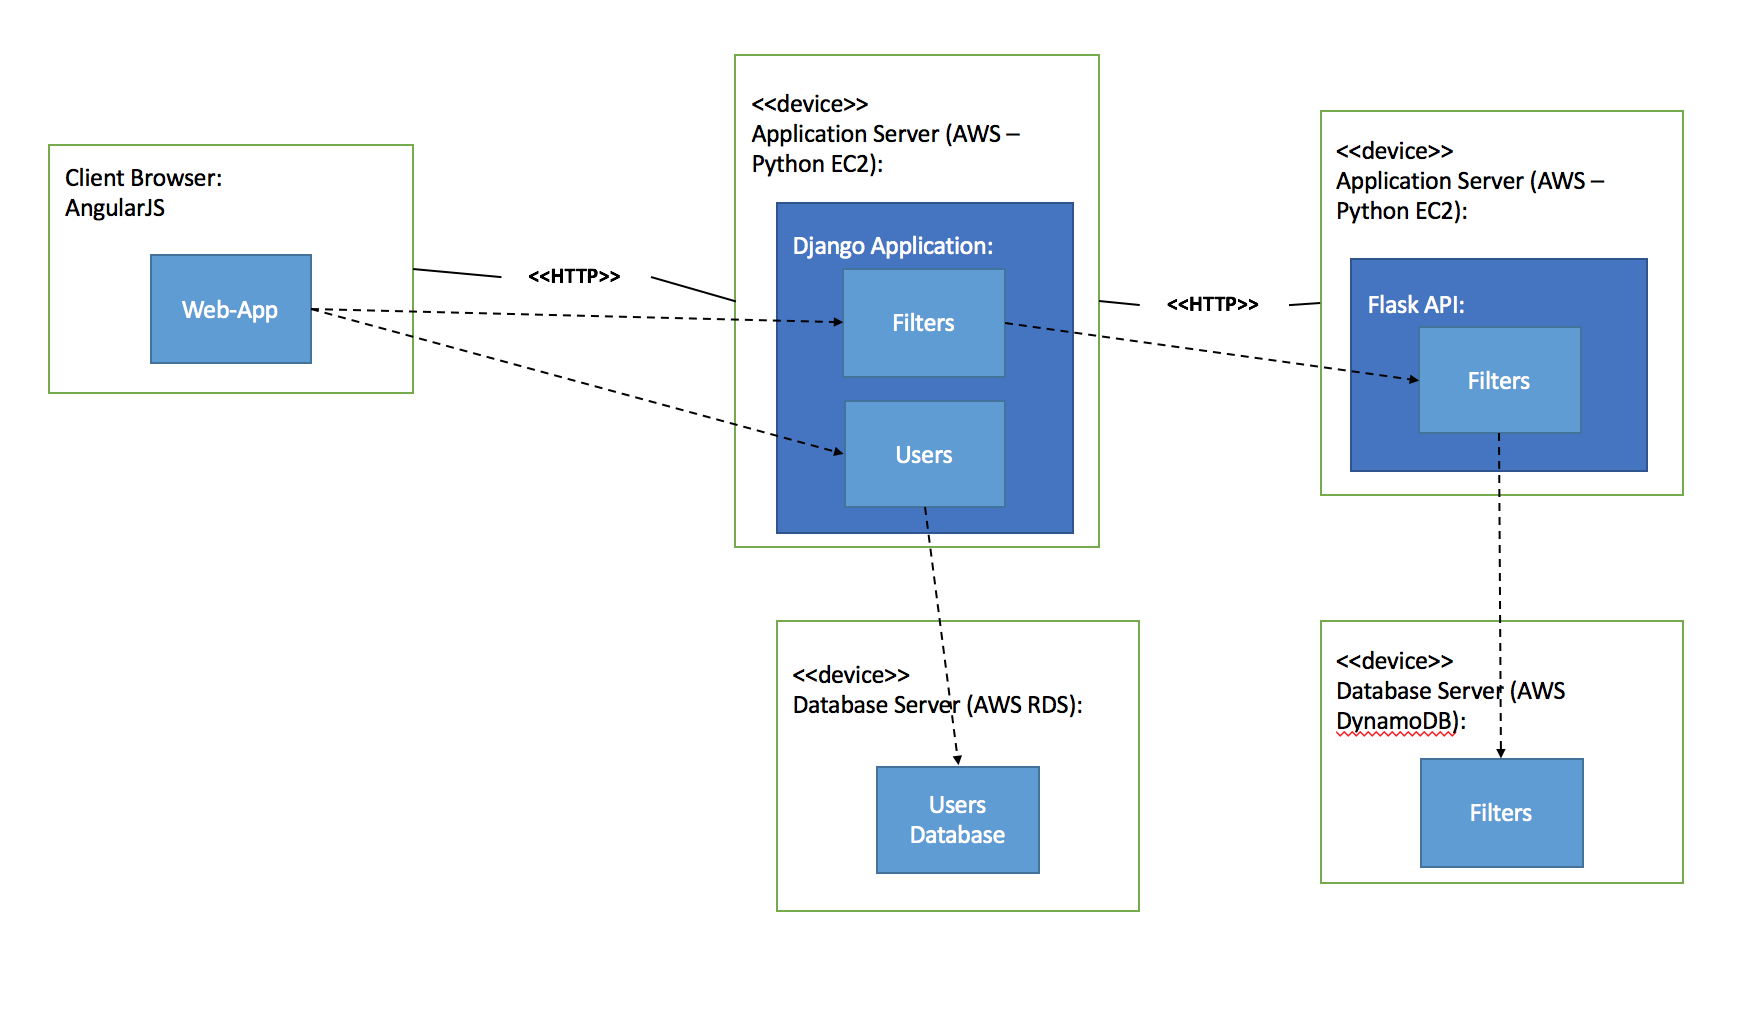
\includegraphics[width=\linewidth]{deployment-diagram}
        \caption{Component deployment diagram}
        \label{fig:deployment-diagram}
      \end{figure}

      Fig. \ref{fig:deployment-diagram} defines the component layout for the entire workflow of the application proposed in this report.

      \subsection{API - AWS}

      \subsection{Front-end - Github Pages}

    \section{Use Case \& Class diagram}

  % \section{Data structures}

\chapter{Implementation} \label{cha:implement}

      \subsection{Other Libraries}

        \subsubsection{NumPy} \label{sec:numpy}

        \subsubsection{SciKit} \label{sec:scikit}

        \subsubsection{Pillow} \label{sec:pillow}

\chapter{Evaluation}
  Within this report there were multiple aims which were set out to be achieved. These aims covered a variety of subjects such as computer vision for image analysis and following best practices for developing an API and Web App. The main of these requirements were developing the API, developing the Web front-end, developing a system for filtering images, and most importantly developing a recommender system for those filters. The system proposed and implemented in chapter \ref{cha:implement} meets most of these goals well, and the evaluation of the product will consist of how well the original objectives set out in section \ref{sec:objectives} were met. The objectives and their evaluations are set out below.

  \newpage
  \subsubsection{Objective \ref{obj1} - Implement a simple online web application for filtering images using a framework or library designed for front-end development across multiple platforms.}
    The front-end propsosed in this report is very effective in its use as an interface on top of the API. It is very lightweight and simple however it is also very functional and robust. The use of React really helped to streamline the development as it meant the structure in the code of the front-end was already much easier to work with. The component structure allows for very easy management of application flow, with variables and callback functions being passed to child components the application is easily able to deal with calling an external API and passing that information to components which automatically update upon recieving that information. However, the requirement for the web app working across multiple platforms was not met. During development the front-end was run purely on a few different desktop browsers such as Safari and Chrome which worked perfectly, however after finally deploying it to a public URL and accessing it from a mobile device it was found that no response came back to the device once an image was uploaded for filtering. Due to the nature of mobile devices there was no easy way to troubleshoot what was going on, where on a desktop device this could easily be done by debugging it in an IDE. Finally, there was not enough time after deploying the application to do an investigation into this issue therefore it can only be viewed as a partial failure to meet one of the objectives.

  \subsubsection{Objective \ref{obj2} - Implement a back-end application which is able to process images including applying filters and creating thumbnails.}
    The python back-end proposed in this report is highly capable of processing images due to the libraries available and its ability to connect easily to the API code. The libraries NumPy and Pillow were both instrumental to the success of image processing, however there was a decent learning curve to both of these along with python itself. This slightly limited how much processing was able to be done on the images as much more time had to be spent researching what libraries are available and what the best practices are for processing images in python. The code design proposed helped very much in how the filters connected to the API, as each filter was a sub-class of a base filter the filters could easily be run by looping through the ‘\texttt{\_\_subclasses\_\_()}’ method on the base class, passing in the ‘\texttt{Filterable}’ object each time. The ‘\texttt{Filterable}’ class also allowed the images to be quickly converted from Pillow types to NumPy types, and also to resize the image into different sizes such as thumbnail and preview sizes.

  \subsubsection{Objective \ref{obj3} - Research various recommender systems to determine the common technologies/solutions for solving the problem of recommendations.}
    In section \ref{sec:lit-recc} various examples of recommender systems were found and a general concensus was discovered that machine learning tools are a very useful tool in recommender systems. While there was not a single blanket solution, and the solutions available are often still not very effective - facing issues such as the cold-start problem which is still a popular research topic. Deep learning was discovered to be a very common tool in industry however this was not feasible due to performance constraints and that they did not seem to be fully applicable to the problem of recommending filters.

  \subsubsection{Objective \ref{obj4} - Implement a recommender system which is able to suggest photo filters to users based on image content.}
    Within this objective the strict definition was met, as a recommender system was built which is able to recommend filters based on image content. However, the accuracy of the AI system which was implemented was not very high, and often came up with highly inconsistent values when producing classification accuracy reports. When using a trained model with a higher trained accuracy of around 35\% on average per class, the model did however seem to have some predictability in how it would recommend filters such as when the photo included one or more faces. The low accuracy would seem to suggest that the method for training the model was not ideal in that users may have had differing tastes for which filters to apply. Furthermore the recommender would occasionally suggest different recommendations when the same photograph was uploaded twice. This is likely a combination of the K-Means analysis producing slightly different results each time and the classifiers not having a strong enough trained model.

  \subsubsection{Objective \ref{obj5} - Implement a RESTful API which exposes both the recommender system and the filtering system to the front-end web app and allows developers to connect them into their own applications.}
    This objective was met easily with the python back-end using the Flask library. This library included helper methods for handling RESTful API's and allowed for doing things such as responding with an ‘\texttt{HTTP 201 CREATED}’ response when a resource was uploaded to the site via an ‘\texttt{HTTP POST}’ request. The URI structure was also within REST constraints, with images being uploaded to the ‘\texttt{/images/}’ URL via an ‘\texttt{HTTP POST}’ request, then being accesed using an ‘\texttt{HTTP GET}’ request from that URL such as\\ ‘\texttt{/images/98119-black\_and\_white.jpg}’. The URI structure was relatively simple due to the simplicity of the request being made therefore it was easier to develop. The responses from the API were also very easy to output as JSON due to python's ability to define a ‘\texttt{dict}’ object using a very similar syntax to JSON, directly in the code. This ‘\texttt{dict}’ object could then easily be translated into an HTTP response using Flask's ‘\texttt{jsonify()}’ method. The API was then easily connected to the front-end and using React which is based in JavaScript made handling JSON responses that much easier, due to JavaScript's high integration with JSON (which makes sense as JSON stands for JavaScript Object Notation...).

\chapter{Conclusion}

\newpage
\singlespacing

\bibliographystyle{agsm}
\bibliography{report}

\end{document}
